% 2022-05-30 Session 27 Rhodes 10 9:00 -- 10:30, presentation 10:15 -- 10:30
% 7. Leipziger Semantic Web Tag, English presentation about the SNIK Quiz.
% 15 minutes presentation.

%\documentclass[aspectratio=43]{beamer}
%\documentclass[aspectratio=169]{beamer}
\documentclass[aspectratio=1610,12pt]{beamer}

\usepackage[english]{babel}
\usepackage{booktabs} % fancy tables
\usepackage{tabulary} % tables with auto column length 
\usepackage{hyperref}
\usepackage{csquotes}
\usepackage{siunitx}
\usepackage{listings}
\usepackage{beramono}% monotype with bold

\usetheme{imise2}
\author{\textbf{Konrad Höffner}, Arne Roszeitis, Max Niclas Wächtler, Franziska Jahn, Prof. Alfred Winter.}
%Institute for Medical Informatics, Statistics and Epidemology. Medical Faculty, Leipzig University, Germany.
%Institute for Medical Informatics, Statistics and Epidemiology}
%\title{The SNIK Ontology of Information Management in Hospitals}
\title{SNIK Quiz: A Multiple Choice Game\\about Information Management in Hospitals}
\date{~}
%\date{May 30, 2022, MIE 2022}
\def\address{Medical Faculty, Leipzig University, Germany.}% Härtelstraße 16-18, 04107 Leipzig, }
\def\email{konrad.hoeffner@imise.uni-leipzig.de} 
\def\telephone{+49 341 97 16322}

\makeatletter
\newcommand*\tableonly%>>>
  {%
    \omit\@ifnextchar<\table@only\table@@only
  }%<<<
\protected\long\def\table@only<#1>#2%>>>
  {%
    \gdef\beamer@doifnotinframe{\cr}%
    \def\beamer@doifinframe{\cr#2}%
    \beamer@masterdecode{#1}%
    \beamer@donow
  }%<<<
\protected\long\def\table@@only#1%>>>
  {%
    \beamer@ifnextcharospec{\table@@@only{#1}}{\cr#1}%
  }%<<<
\long\def\table@@@only#1<#2>%>>>
  {%
    \gdef\beamer@doifnotinframe{\cr}%
    \def\beamer@doifinframe{\cr#1}%
    \beamer@masterdecode{#2}%
    \beamer@donow
  }%<<<
\makeatother

\newcommand{\imageslide}[4][]
{
\newgeometry{margin=0cm,top=1em}
\begin{frame}[plain]{~~~~#2}
\vspace{0.2em}
\centering\includegraphics[width=1.0\textwidth,height=0.95\textheight,keepaspectratio]{#3}
\\#1
\note{#4}
\end{frame}
\restoregeometry
}

\begin{document}
{
\iffalse
\setbeamertemplate{background canvas}%
{
 \vbox to \paperheight{\vfil\hbox to \paperwidth{%
 \hfil 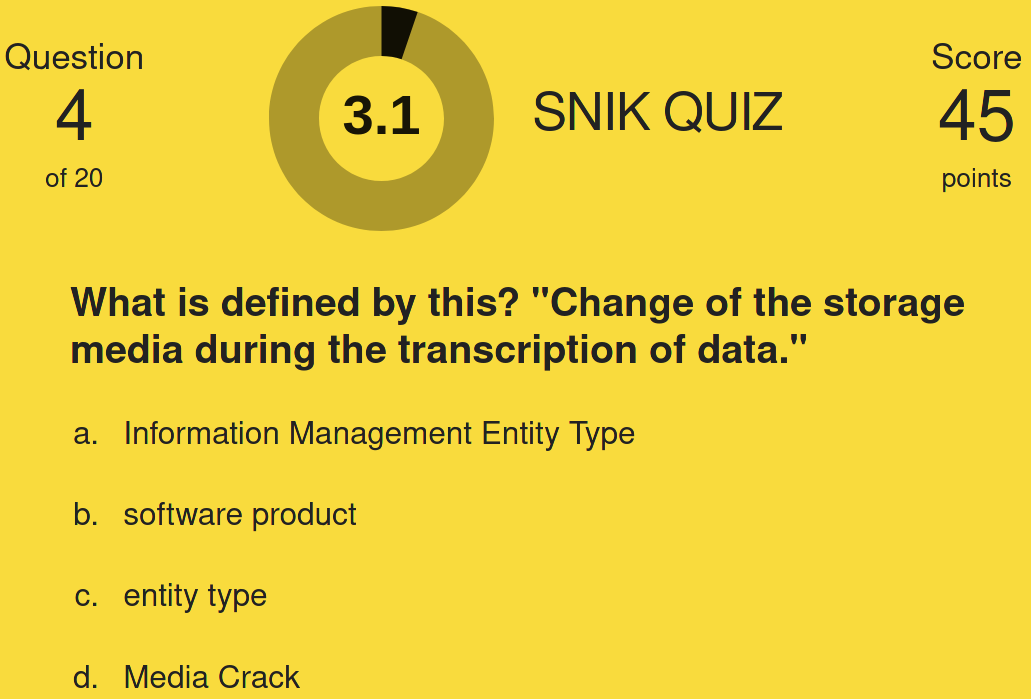
\includegraphics[width=\paperwidth,height=\paperheight,keepaspectratio]{img/snik-quiz.png} \hfil}
 }
}
\fi
\begin{frame}
\titlepage
\end{frame}
}


\newgeometry{margin=0cm,top=1em}
\begin{frame}[plain]{~~~~Information Management in Hospitals}
% Information Management in Hospitals is a core topic for students of medical computer science.
% Unfortunately, there are many different views of the domain, whose relationship is often unclear, and the terminology is full of synonyms and homonyms.
% So this domain is difficult to learn for students. 
\centering\includegraphics[height=0.77\textheight,keepaspectratio]{img/book-bb.jpg}
\centering\includegraphics[height=0.77\textheight,keepaspectratio]{img/book-ob.jpg}
\centering\includegraphics[height=0.77\textheight,keepaspectratio]{img/book-he.jpg}
\end{frame}
\restoregeometry

\imageslide{}{img/snik-quiz.png}{}{}

%\imageslide{Vocabulary}{img/wordcloud-ob.png}{}{}
%\imageslide{Synonyms}{img/wordcloud-synonym.png}{}{}

\newgeometry{margin=0cm,top=1em}
\begin{frame}[plain]{~~SNIK: Semantic Network of Information Management in Hospitals}
\centering\includegraphics[height=0.21\textheight,keepaspectratio]{img/book-bb.jpg}
\centering\includegraphics[height=0.21\textheight,keepaspectratio]{img/book-ob.jpg}
\centering\includegraphics[height=0.21\textheight,keepaspectratio]{img/book-he.jpg}
\centering\includegraphics[width=0.7\textwidth,keepaspectratio]{img/5star.png}
\end{frame}
\restoregeometry

\imageslide{SNIK Meta Model}{img/metamodel9s.pdf}{}{}
\imageslide{Class Hierarchy Excerpt}{img/bb-cio.pdf}{}{}

\imageslide{SNIK}{img/snik-graph-full.png}{}{}

\iffalse
\begin{frame}{Multiple Choice Question Components}
\begin{itemize}
\item Question Stem
\item Key: Correct Answer
\item Distractors: Incorrect Answers
\end{itemize}
\end{frame}
\fi

\imageslide{Multiple Choice Question Components}{img/snik-quiz-annotated.png}{}{}

\begin{frame}[fragile]{Simple Question Templates}
\begin{tabulary}{\textwidth}{lL}
\toprule
\textbf{Template}	&\textbf{Description}\\
\midrule
\tableonly<1>{
\textbf{Subject}		&Ask for the subject of a (subject, relation, object) triple given the relation and object.\\
%						&Distractors are labels of other classes (of the same type) that \emph{are not} related via the same relation to the same object but which are connected to the correct answer with a path of length at most 2.\\
Stem					&\emph{Who is responsible for Medical Admission?}\\
Key						&\emph{Physician}\\
Distractors				&\emph{Surgeon}, \emph{Health Care Professional}, \emph{Senior Physician}\\
}
\tableonly<2>{
\textbf{Object}			&Ask for the object of a (subject, relation, object) triple given the subject and relation.\\
Stem					&\emph{The Specification Team is responsible for}$\ldots$\\
Key						&\emph{Functional Specification Document}\\
Distractors: 			&\emph{Project Team Member}, \emph{Sponsor}, \emph{Defining Project Organization}\\
}
\tableonly<3>{
\textbf{Definition}		&Ask for the entity that fits the given textbook definition.\\
Stem					&\emph{What is defined by this? \enquote{X assures a defined quality of all processes and outcomes of the hospital}}\\
Key						&\emph{Internal Quality Management}\\
Distractors				&\emph{Activity}, \emph{Complaint}, \emph{Diagnosis}\\
}
\tableonly<4>{
\textbf{Definitions}	&Present different definitions and ask, which of them fits the given entity.\\
Stem					&\emph{What defines the term Data Warehouse System?}\\
Key						&\emph{Application component that contains data which have been extracted from other application components, in order to support either hospital management or clinical research.}\\
Distractors				&\emph{Defines the hospital’s long-term strategic goals},
						\emph{An application component where the controlling rules for data processing are implemented as executable software},
						\emph{Summarizes monitored key performance indicators (KPIs) and compares them to the expected future state}\\
}
\bottomrule
\end{tabulary}
\end{frame}

\begin{frame}[fragile]{Complex Question Templates}
\begin{tabulary}{\textwidth}{lL}
\toprule
\textbf{Template}	&\textbf{Description}\\
\midrule
\tableonly<1>{
\textbf{Intertwined}	&The correct answer and distractors are more strongly connected.\\
Stem					&\emph{In the context of Strategic Information Management, which one of the following triples belongs together the most?}\\
Key						&\emph{Chief Information Officer -- Department of Information management -- IM Staff}\\
Distractor 1			&\emph{Chief Information Officer -- Strategic Gap -- Corporate Strategy}\\
Distractor 2			&\emph{Chief Information Officer -- Ticket Evaluation -- Project Monitoring}\\
}
\tableonly<2>{
\textbf{Occurence}		&Ask whether a given term is defined in one two textbooks, both or neither.\\
Stem					&\emph{In which contexts does the term \enquote{Health Insurance Company} occur?}\\
Key						&\emph{Strategic Information Management}\\
Distractors				&\emph{Tactical Information Management, Both Contexts, Neither}\\
}
\tableonly<3>{
\textbf{CloseMatch}		&Transfer knowledge about one textbook to the other by confirming or denying statements about entity pairs that are marked as near equivalent.\\
Stem					&\emph{In the Strategic Information Management, the Consultant is associated with the Long-Term HIS Planning, while in the Tactical Information Management, the Consultant is responsible for the Functional Specification Document.} (Key: True, Distractor: False)\\
}
\bottomrule
\end{tabulary}
\end{frame}

\begin{frame}[fragile]{SPARQL Query for Definition questions}
\begin{lstlisting}[basicstyle=\footnotesize,breaklines=true,escapeinside={(*}{*)}]
SELECT SAMPLE(REPLACE(STR(?def),STR(?cl),"X","i") AS ?def) SAMPLE(STR(?cl) AS ?cl) SAMPLE(STR(?a1l) AS ?a1l) SAMPLE(STR(?a2l) AS ?a2l) SAMPLE(STR(?a3l) AS ?a3l) {
  ?class a owl:Class; rdfs:label ?cl.
  FILTER(LANGMATCHES(LANG(?cl),"en"))
  (*\bfseries ?class skos:definition ?def.*)
  FILTER(STRLEN(?def)>10&&STRLEN(?def)<600).
  FILTER(LANGMATCHES(LANG(?def),"en"))
  (*\bfseries ?class (!(meta:subTopClass$|$rdf:type))\{1,2\} ?a1,?a2,?a3.*)
  owl:Class ^a ?a1,?a2,?a3.
  (*\bfseries FILTER(?class!=?a1\&\&?class!=?a2\&\&?class!=?a3\&\&?a1<?a2\&\&?a2<?a3)*)
  ?a1 rdfs:label ?a1l. FILTER(LANGMATCHES(LANG(?a1l),"en"))
  ?a2 rdfs:label ?a2l. FILTER(LANGMATCHES(LANG(?a2l),"en"))
  ?a3 rdfs:label ?a3l. FILTER(LANGMATCHES(LANG(?a3l),"en"))
} GROUP BY ?class LIMIT 1000
\end{lstlisting}
\end{frame}

\begin{frame}[fragile]{Limitations and Future Work}
\begin{figure}
\centering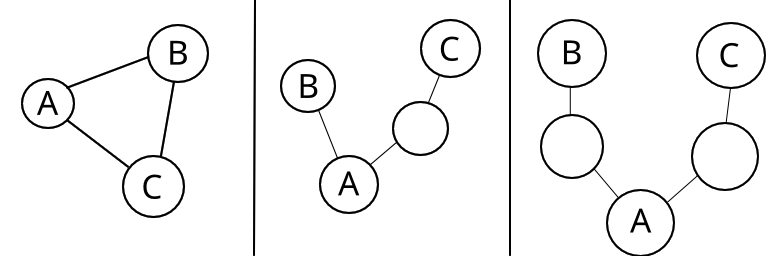
\includegraphics[height=0.3\textheight,keepaspectratio]{img/intertwined_cml.png}
\caption{Key, difficult and easy distractor for intertwined questions.}
\end{figure}
\begin{itemize}
%\item programmers, Semantic Web experts, domain experts, teachers
\item intertwined questions based on graph structure that is not relevant to users
\item didactic value of complex templates questionable\pause
\item early introduction of domain experts and didactic methods needed\pause
\item identify relevant criteria and perform systematic evaluation on large group of students
\end{itemize}
\end{frame}

\begin{frame}[fragile]{Questions?}
\begin{itemize}
%\item Diese Präsentation \url{https://github.com/KonradHoeffner/latex/releases/download/colloquium/colloquium.pdf}
\vspace{0.5em}%here it works as intended
\item Quiz Prototype \url{http://www.snik.eu/quiz}
\item GitHub \url{https://github.com/snikproject/quiz}
\item Ontology\url{https://github.com/snikproject/ontology}
\item SPARQL Endpoint \url{http://www.snik.eu/sparql}
\item SNIK Website \url{http://www.snik.eu}
\item Graph Visualization \url{http://www.snik.eu/graph}
\item RDF Browser \url{http://www.snik.eu/ontology}
\item Paper Preprint \url{https://www.snik.eu/public/snik-quiz-mie2022.pdf}
\item Bachelor Thesis: Arne Roszeitis \emph{Automatische Generierung komplexer Fragen zum Informationsmanagement auf der Basis der SNIK-Ontologie} (German); 2022. \url{https://www.snik.eu/public/bachelor-ar.pdf}
\end{itemize}
\end{frame}

\end{document}
